\documentclass[12pt]{article}
\usepackage{tikz}
\usepackage{collcell}
\usepackage{xcolor}
\usepackage{pgf}

% Define the minimum and maximum values for gradient coloring
\newcommand*{\MinValue}{0}%
\newcommand*{\MaxValue}{100}%

% Apply gradient coloring based on the value
\newcommand{\ApplyGradient}[1]{%
    \pgfmathsetmacro{\PercentColor}{(#1-\MinValue)/(\MaxValue-\MinValue)*100}
    \hspace{-0.33em}\colorbox{red!\PercentColor!green}{\textcolor{black}{#1}}
}

\newcolumntype{R}{>{\collectcell\ApplyGradient}c<{\endcollectcell}}
\renewcommand{\arraystretch}{0}
\setlength{\fboxsep}{3mm} % box size
\setlength{\tabcolsep}{0pt}


% PCA reconstructed Iothers delta frequency %

\begin{document}
\begin{table}[ht]
\centering
\caption{PCA reconstructed Iothers delta frequency}
\vspace{10pt} % Add more space here
\begin{tabular}{c *{5}{R}}
\multicolumn{1}{c}{} & \multicolumn{1}{c}{Matched} & \multicolumn{1}{c}{One-Head} & \multicolumn{1}{c}{One-Data} & \multicolumn{1}{c}{Random} & \multicolumn{1}{c}{Sensor} \\
AECno ort & 0.0000 & 0.0000 & 0.0000 & 0.0000 & 0.0780 \\
AECort & 0.0000 & 0.0000 & 0.0000 & 0.0000 & 0.0841 \\
ciPLV &  0.1069 & 0.1389 & 0.0253 & 0.1199 & 0.1441\\
\end{tabular}

% Color Scale
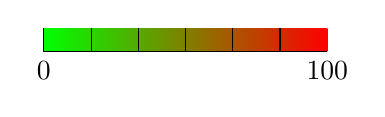
\begin{tikzpicture}[scale=0.6]
    \fill[left color=green, right color=red] (0,0) rectangle (6,0.5);
    \draw (0,0) -- (6,0);
    \foreach \x in {0,20,...,100}
        \draw ({\x/20},0) -- ({\x/20},0.5);
    \node[below] at (0,0) {\MinValue};
    \node[below] at (6,0) {\MaxValue};
\end{tikzpicture}
\end{table}

% PCA reconstructed Iothers theta frequency %

\begin{table}[ht]
\centering
\caption{PCA reconstructed Iothers theta frequency}
\vspace{10pt} % Add more space here
\begin{tabular}{c *{5}{R}}
\multicolumn{1}{c}{} & \multicolumn{1}{c}{Matched} & \multicolumn{1}{c}{One-Head} & \multicolumn{1}{c}{One-Data} & \multicolumn{1}{c}{Random} & \multicolumn{1}{c}{Sensor} \\
AECno ort & 0.0000 & 0.0000 & 0.0000 & 0.0000 & 0.1272 \\
AECort & 0.0000 & 0.0000 & 0.0000 & 0.0000 & 0.0888 \\
ciPLV &  0.0891 & 0.1451 & 0.0605 & 0.1123 & 0.1276\\
\end{tabular}

% Color Scale
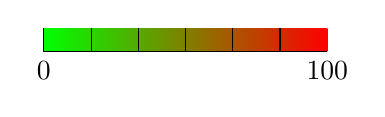
\begin{tikzpicture}[scale=0.6]
    \fill[left color=green, right color=red] (0,0) rectangle (6,0.5);
    \draw (0,0) -- (6,0);
    \foreach \x in {0,20,...,100}
        \draw ({\x/20},0) -- ({\x/20},0.5);
    \node[below] at (0,0) {\MinValue};
    \node[below] at (6,0) {\MaxValue};
\end{tikzpicture}
\end{table}

% PCA reconstructed Iothers alpha frequency %

\begin{table}[ht]
\centering
\caption{PCA reconstructed Iothers alpha frequency}
\vspace{10pt} % Add more space here
\begin{tabular}{c *{5}{R}}
\multicolumn{1}{c}{} & \multicolumn{1}{c}{Matched} & \multicolumn{1}{c}{One-Head} & \multicolumn{1}{c}{One-Data} & \multicolumn{1}{c}{Random} & \multicolumn{1}{c}{Sensor} \\
AECno ort & 0.0000 & 0.0000 & 0.0000 & 0.0000 & 0.1985  \\
AECort & 0.0000 & 0.0000 & 0.0000 & 0.0000 & 0.1611 \\
ciPLV & 0.0898 & 0.1510 & 0.0421 & 0.0758 & 0.1362\\
\end{tabular}

% Color Scale
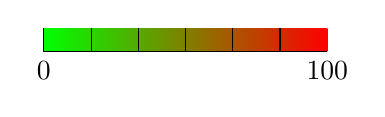
\begin{tikzpicture}[scale=0.6]
    \fill[left color=green, right color=red] (0,0) rectangle (6,0.5);
    \draw (0,0) -- (6,0);
    \foreach \x in {0,20,...,100}
        \draw ({\x/20},0) -- ({\x/20},0.5);
    \node[below] at (0,0) {\MinValue};
    \node[below] at (6,0) {\MaxValue};
\end{tikzpicture}
\end{table}


% PCA reconstructed Iothers beta frequency %

\begin{table}[ht]
\centering
\caption{PCA reconstructed Iothers beta frequency}
\vspace{10pt} % Add more space here
\begin{tabular}{c *{5}{R}}
\multicolumn{1}{c}{} & \multicolumn{1}{c}{Matched} & \multicolumn{1}{c}{One-Head} & \multicolumn{1}{c}{One-Data} & \multicolumn{1}{c}{Random} & \multicolumn{1}{c}{Sensor} \\
AECno ort & 0.0000 & 0.0000 & 0.0000 & 0.0000 & 0.1951 \\
AECort & 0.0000 & 0.0000 & 0.0000 & 0.0000 & 0.1738\\
ciPLV &  0.0925 & 0.1551 & 0.0591 & 0.1001 & 0.1628\\
\end{tabular}

% Color Scale
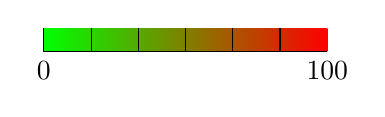
\begin{tikzpicture}[scale=0.6]
    \fill[left color=green, right color=red] (0,0) rectangle (6,0.5);
    \draw (0,0) -- (6,0);
    \foreach \x in {0,20,...,100}
        \draw ({\x/20},0) -- ({\x/20},0.5);
    \node[below] at (0,0) {\MinValue};
    \node[below] at (6,0) {\MaxValue};
\end{tikzpicture}
\end{table}


% PCA reconstructed Iothers gamma frequency %

\begin{table}[ht]
\centering
\caption{PCA reconstructed Iothers gamma frequency}
\vspace{10pt} % Add more space here
\begin{tabular}{c *{5}{R}}
\multicolumn{1}{c}{} & \multicolumn{1}{c}{Matched} & \multicolumn{1}{c}{One-Head} & \multicolumn{1}{c}{One-Data} & \multicolumn{1}{c}{Random} & \multicolumn{1}{c}{Sensor} \\
AECno ort & 0.0000 & 0.0000 & 0.0000 & 0.0000 & 0.1620\\
AECort & 0.0000 & 0.0000 & 0.0000 & 0.0000 &  0.1837\\
ciPLV &  0.0815 & 0.1441 & 0.0379 & 0.1235 & 0.1611\\
\end{tabular}

% Color Scale
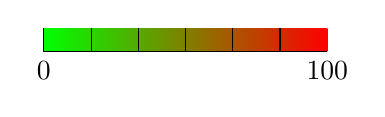
\begin{tikzpicture}[scale=0.6]
    \fill[left color=green, right color=red] (0,0) rectangle (6,0.5);
    \draw (0,0) -- (6,0);
    \foreach \x in {0,20,...,100}
        \draw ({\x/20},0) -- ({\x/20},0.5);
    \node[below] at (0,0) {\MinValue};
    \node[below] at (6,0) {\MaxValue};
\end{tikzpicture}
\end{table}
\end{document}
